\documentclass[xcolor=table]{beamer}
\usepackage{fontspec}
\usepackage{natbib}
\usepackage{polyglossia} 
\usepackage[table]{xcolor}
\usepackage{gb4e} 
\usepackage{booktabs} 
\usepackage{multicol,multirow}
\usepackage{color}
%\usepackage{colortbl}
\usepackage{graphicx}
  \setmainfont[Mapping=tex-text]{Charis SIL}
\let\sfdefault\rmdefault
\newcommand{\racine}[1]{\begin{math}\sqrt{#1}\end{math}} 
\newcommand{\grise}[1]{\cellcolor{lightgray}\textbf{#1}} 
\usepackage{epsf}
   \newcommand{\ra}{$\Sigma_1$} 
\newcommand{\rc}{$\Sigma_3$} 
\newcommand{\ro}{$\Sigma$} 
\newfontfamily\phon[Mapping=tex-text,Ligatures=Common,Scale=MatchLowercase,FakeSlant=0.3]{Charis SIL} 
\newcommand{\rouge}[1]{{\color{red}#1}}
\newcommand{\bleu}[1]{{\color{blue}#1}}
 \newcommand{\ipa}[1]{{\phon #1}} %API tjs en italique
\newfontfamily\phondroit[Mapping=tex-text,Ligatures=Common,Scale=MatchLowercase]{Charis SIL} 
\newcommand{\ipapl}[1]{{\phondroit #1}} 
\newfontfamily\cn[Mapping=tex-text,Ligatures=Common,Scale=MatchUppercase]{MingLiU}%pour le chinois
\newcommand{\zh}[1]{{\cn #1}}

\newcommand{\subone}{₁}
\newcommand{\subtwo}{₂}
\newcommand{\agent}{\textsc{a}}
\newcommand{\abl}{\textsc{abl}}
\newcommand{\abs}{\textsc{abs}}
\newcommand{\acc}{\textsc{acc}}
\newcommand{\addr}{\textsc{addr}}
\newcommand{\adn}{\textsc{adn}}
\newcommand{\allat}{\textsc{all}}
\newcommand{\alloc}{\textsc{alloc}}
\newcommand{\art}{\textsc{art}}
\newcommand{\asp}{\textsc{asp}}
\newcommand{\assert}{\textsc{decl}}
\newcommand{\aor}{\textsc{aor}}
\newcommand{\auth}{\textsc{auth}}
\newcommand{\aux}{\textsc{aux}}
\newcommand{\cnv}{\textsc{cnv}}
\newcommand{\comp}{\textsc{comp}}
\newcommand{\concess}{\textsc{concess}}
\newcommand{\cond}{\textsc{cond}}
\newcommand{\conv}{\textsc{cvb}}
\newcommand{\const}{\textsc{testim}}
\newcommand{\cop}{\textsc{cop}}
\newcommand{\dest}{\textsc{dest}}
\newcommand{\dat}{\textsc{dat}}
\newcommand{\deb}{\textsc{deb}}
\newcommand{\defin}{\textsc{def}}
\newcommand{\defer}{\textsc{defer}}
\newcommand{\dem}{\textsc{dem}}
\newcommand{\dep}{\textsc{dep}}
\newcommand{\determ}{\textsc{det}}
\newcommand{\elat}{\textsc{el}}
\newcommand{\emphat}{\textsc{emph}}
\newcommand{\equat}{\textsc{equat}}
\newcommand{\erg}{\textsc{erg}}
\newcommand{\evid}{\textsc{evid}}
\newcommand{\excl}{\textsc{excl}}
\newcommand{\exclam}{\textsc{exclam}}
\newcommand{\fem}{\textsc{f}}
\newcommand{\familier}{\textsc{fam}}
\newcommand{\fin}{\textsc{fin}}
\newcommand{\foc}{\textsc{foc}}
\newcommand{\fut}{\textsc{fut}}
\newcommand{\gen}{\textsc{gen}}
\newcommand{\ger}{\textsc{ger}}
\newcommand{\hon}{\textsc{hon}}
\newcommand{\hort}{\textsc{hort}}
\newcommand{\hum}{\textsc{hum}}
\newcommand{\hyp}{\textsc{hyp}}
\newcommand{\imp}{\textsc{imp}}
\newcommand{\imprf}{\textsc{imprf}}
\newcommand{\inch}{\textsc{incho}}
\newcommand{\incl}{\textsc{incl}}
\newcommand{\ind}{\textsc{ind}}
\newcommand{\indef}{\textsc{indef}}
\newcommand{\infin}{\textsc{inf}}
\newcommand{\instr}{\textsc{instr}}
\newcommand{\inter}{\textsc{inter}}
\newcommand{\inv}{\textsc{inv}}
\newcommand{\loc}{\textsc{loc}}
\newcommand{\masc}{\textsc{m}}
%\newcommand{\mod}{\textsc{mod}}
\newcommand{\negate}{\textsc{neg}}
\newcommand{\neut}{\textsc{n}}
\newcommand{\nmlz}{\textsc{nmlz}}
\newcommand{\nom}{\textsc{nom}}
\newcommand{\oblique}{\textsc{obl}}
\newcommand{\opt}{\textsc{opt}}
\newcommand{\partit}{\textsc{part}}
\newcommand{\pat}{\textsc{p}}
\newcommand{\pl}{\textsc{pl}}
\newcommand{\poss}{\textsc{poss}}
\newcommand{\pot}{\textsc{pot}}
\newcommand{\prev}{\textsc{pv}}
\newcommand{\prf}{\textsc{prf}}
\newcommand{\prox}{\textsc{prox}}
\newcommand{\prs}{\textsc{prs}}
\newcommand{\prt}{\textsc{prt}}
\newcommand{\pass}{\textsc{pass}}
\newcommand{\past}{\textsc{pst}}
\newcommand{\pref}{\textsc{pref}}
\newcommand{\prog}{\textsc{prog}}
\newcommand{\ptcp}{\textsc{ptcp}}
\newcommand{\quot}{\textsc{quot}}
%\newcommand{\rad}{\textsc{rad}}
\newcommand{\refl}{\textsc{refl}}
\newcommand{\rel}{\textsc{rel}}
\newcommand{\resp}{\textsc{rsp}}
\newcommand{\seq}{\textsc{seq}}
\newcommand{\sg}{\textsc{sg}}
\newcommand{\simil}{\textsc{simil}}
\newcommand{\subj}{\textsc{subj}}
\newcommand{\topic}{\textsc{top}}
\newcommand{\tranz}{\textsc{tr}}
\newcommand{\unique}{\textsc{s}}
\newcommand{\voc}{\textsc{voc}}
\begin{document} 
\begin{frame} 

\title{Hybrid indirect speech in Japhug} 

 \author{Guillaume Jacques, CNRS-CRLAO \\ Anton Antonov, INALCO-CRLAO }
\maketitle
 \end{frame} 


\section{Introduction}
\begin{frame}
\frametitle{The Rtau language}


\begin{itemize}
 \item  Rtau (locally known as \ipa{rəsɲəske}) is a Rgyalrongic language spoken in Rtau county (\zh{道孚县} Dàofú xiàn), Sichuan province (\zh{四川省} Sìchuān shěng), China.

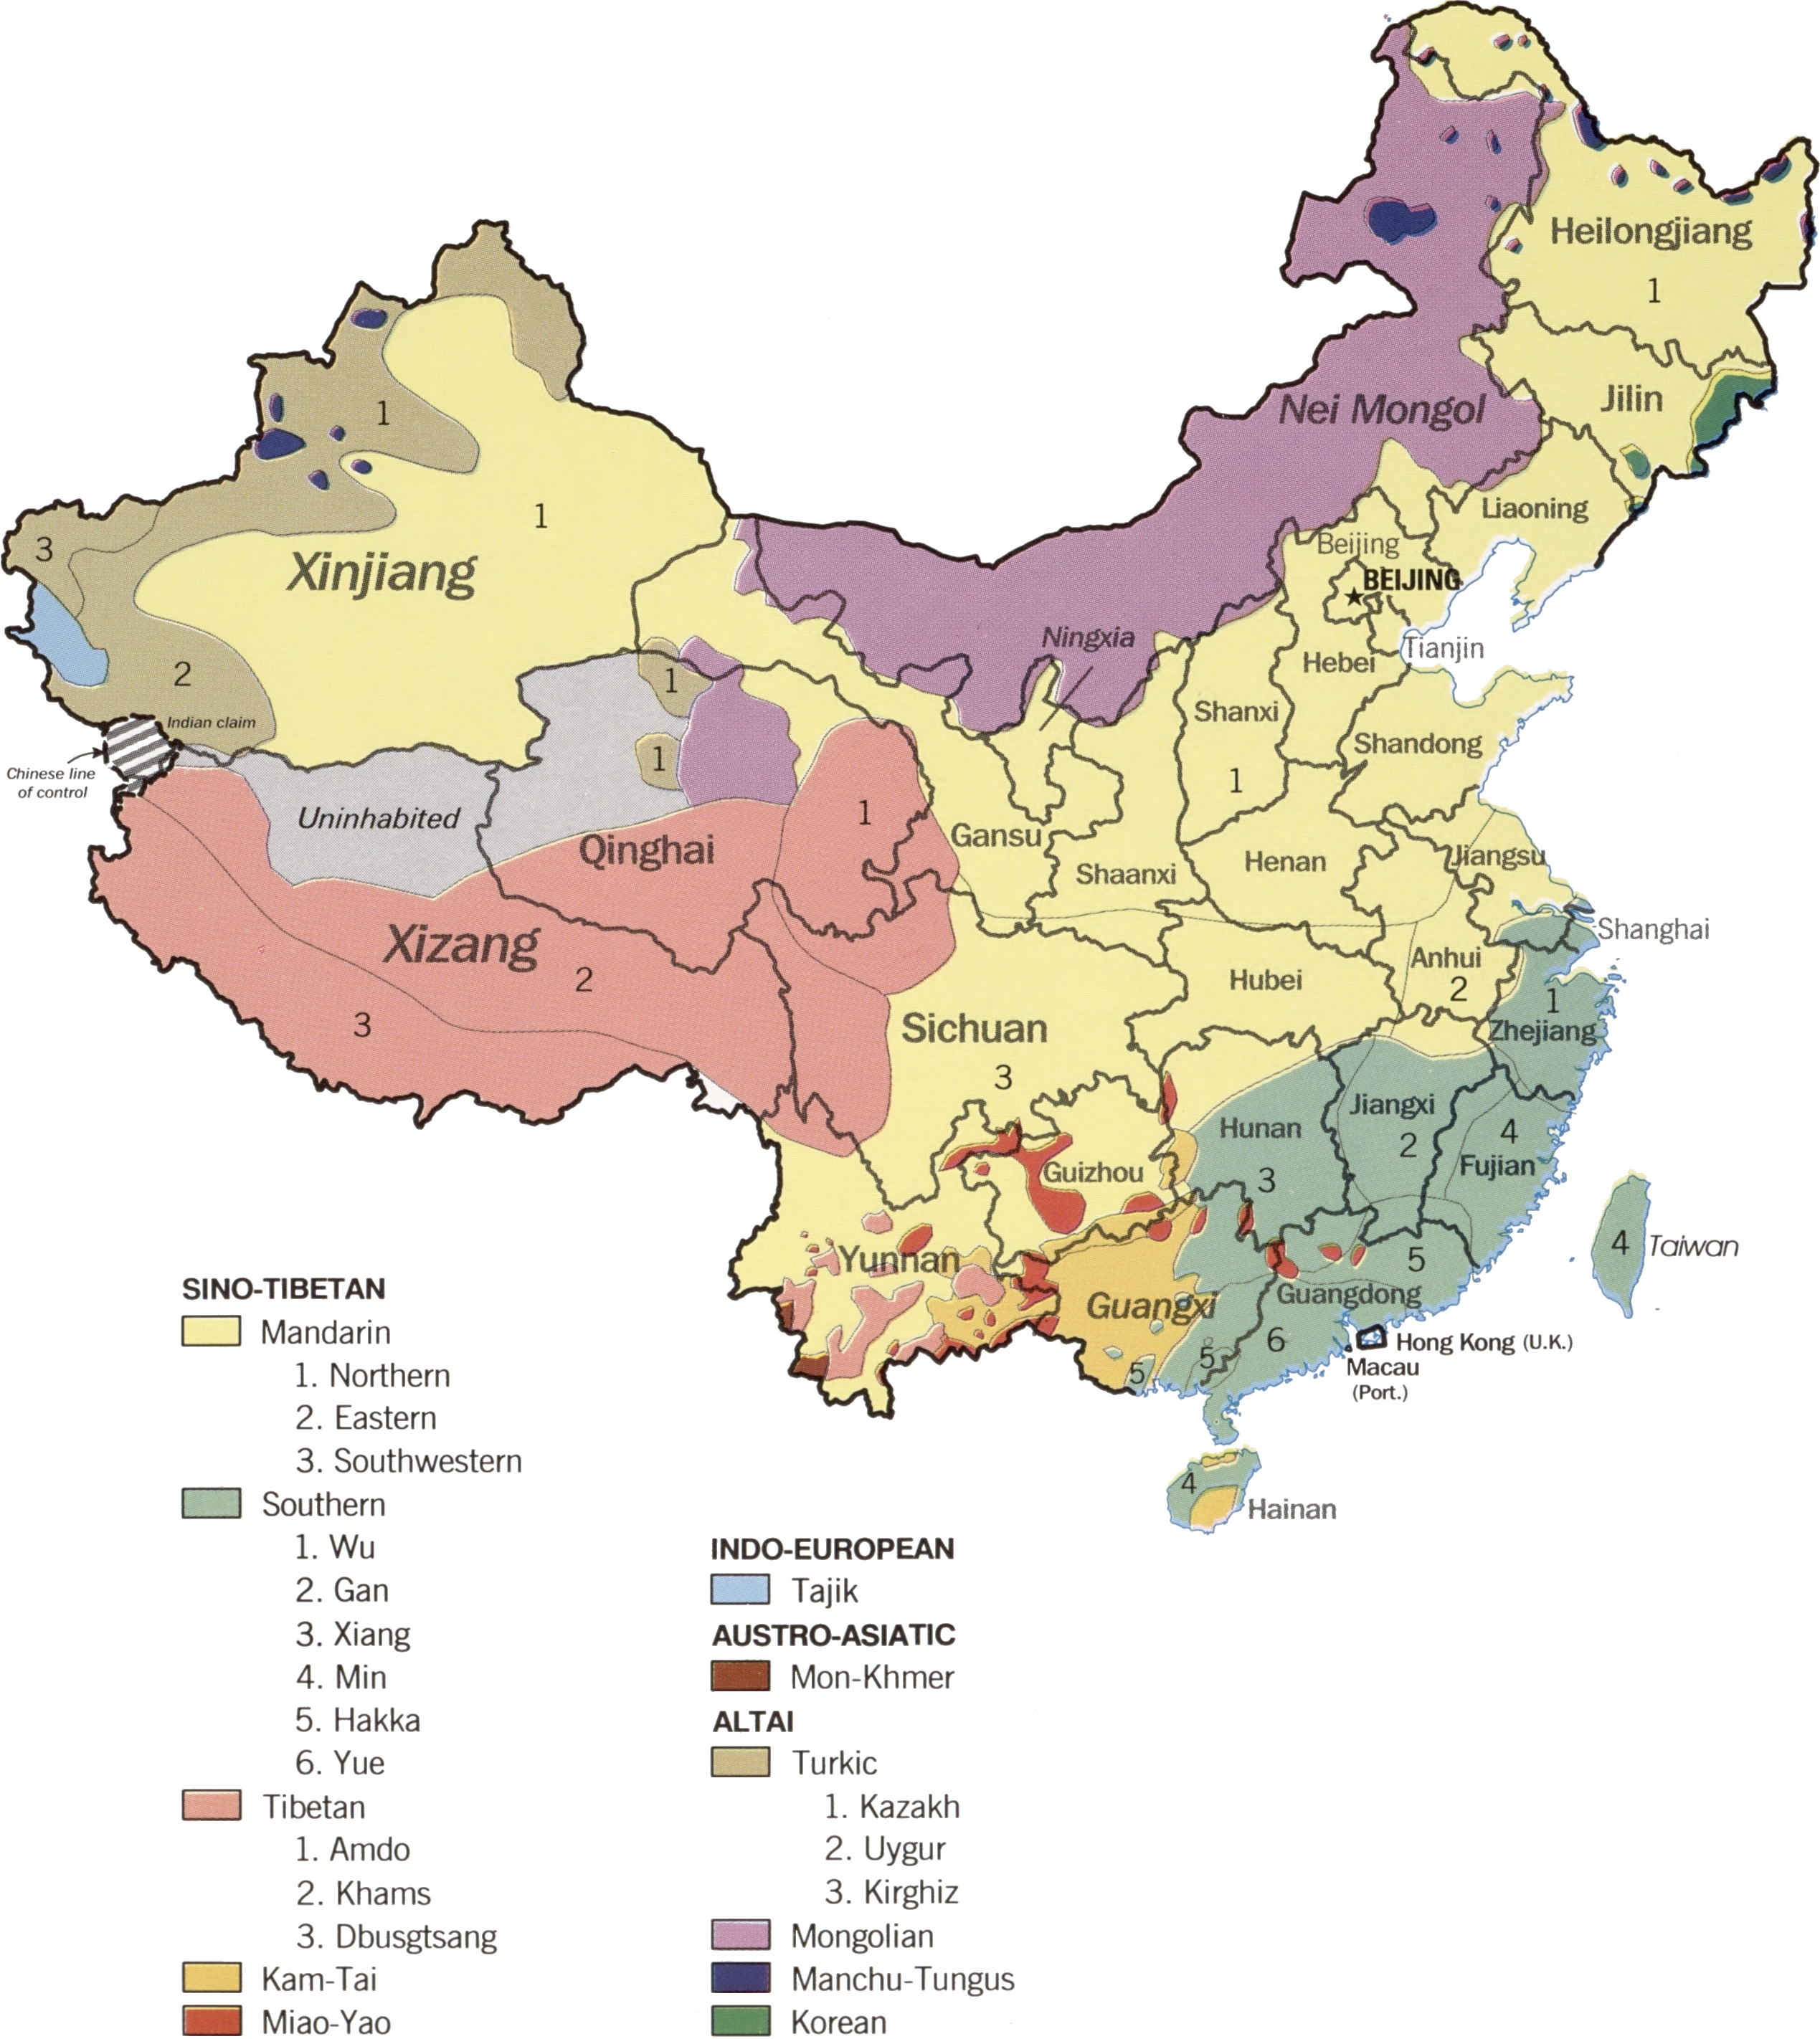
\includegraphics[width=0.5\textwidth]{chinalingmap.jpg}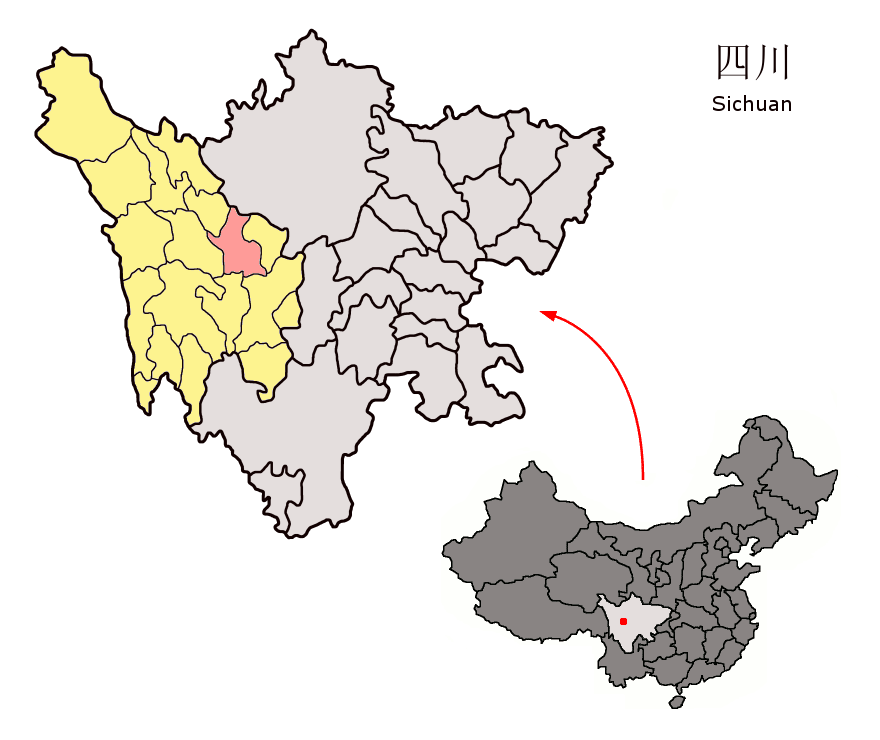
\includegraphics[width=0.5\textwidth]{dawu.png}

\end{itemize}
\end{frame} 


\begin{frame}%[shrink=10]
\frametitle{Person marking and flagging}

\begin{exe}
\ex \label{ex:np3}
\gll
	\ipa{tʂaɕi-w} \ipapl{dʐʚma} 	\ipapl{de} \ipapl{nə-f-se(-sə)} \\
	{Bkrashis-\erg} Sgrolma {\dem} {\prf-\inv-kill(-\evid)}\\ 
	\glt Bkrashis killed Sgrolma.
\end{exe}

\begin{exe}
\ex \label{ex:33}
\gll
	\ipa{tə-w} \ipapl{dʐʚma} \ipapl{de} \ipapl{nə-f-se(-sə)} \\
	{3\sg-\erg} Sgrolma {\dem} {\prf-\inv-kill(-\evid)}\\ 
	\glt He killed Sgrolma.
\end{exe}

\begin{exe}
\ex \label{ex:13}
\gll
	\ipa{ŋa}	\ipapl{dʐʚma} 	\ipapl{de} 	\ipapl{nə-se-w} \\
	{1\sg} Sgrolma {\dem} {\prf-kill-1\sg>3}\\ 
	\glt I killed Sgrolma.
\end{exe}

\begin{exe}
\ex \label{ex:23}
\gll
	\ipa{ɲi}	\ipapl{dʐʚma} 	\ipapl{de} 	\ipapl{nə-se-j(-sə)} \\
	{2\sg} Sgrolma {\dem} {\prf-kill-2\sg>3(-\evid)}\\ 
	\glt You killed Sgrolma.
\end{exe}

\end{frame}


\begin{frame}
 
\begin{itemize}
 \item It is important to note that contrary to what happens in some other Sino-Tibetan languages (esp. in Tibetan languages and some other members of the Rgyalrongic branch) ergative marking is normally blocked on \textsc{sap}.%, with \textsc{sds} being the only exception as far as the first person singular is concerned (the second person singular pronoun remains unmarked as usual as in \ref{ex:1ebis}).
\end{itemize}

\end{frame}

\section{Defining the topic}

\begin{frame}%[shrink=15]
\frametitle{Semi-direct speech}

\begin{itemize}

\item In Rtau, there are two main ways of reporting what someone else has said, direct speech (\textsc{ds}) and semi-direct speech (\textsc{sds}, cf. \citealp{aikhenvald08semidirect}, also called `hybrid speech' by \citealp{tournadre08conjunct}). 

%\item Unlike direct speech, \textsc{sds} is framed by a converbal form and an appropriately conjugated form of the reporting verb \ipa{jə} `say'

\item We have been unable to ascertain the existence of any other type of reported speech, such as indirect speech (\textsc{is}) which is reported to be unattested in Tibetan languages as well (\citealp{tournadre08conjunct}).

\end{itemize}

\end{frame}

\begin{frame}%[shrink=10]
\frametitle{Semi-direct speech}

 

\begin{exe}
\ex \label{ex:1b}
\gll
	\ipa{tʂaɕi-w}$_i$ \ipa{ŋa-gi}	\ipa{jə-rə-ge} [\ipapl{tə-w}$_j$	\ipapl{dʐʚma} 	\ipapl{de} \ipapl{nə-f-se-sə}] \ipa{jə-rə}  \\
	{Bkrashis-\erg} {1\sg-\dat} {say-\const-\conv} {3\sg-\erg} Sgrolma {\dem} {\prf-\inv-kill-\evid}  say-\const\\ 
	\glt Bkrashis$_i$ told me (that) he$_j$ ($\ne$ Bkrashis) had killed Sgrolma.
\end{exe}

\begin{exe}
\ex \label{ex:1c}
\gll
	\ipa{tʂaɕi-w}$_i$ \ipa{ŋa-gi}	\ipa{jə-rə-ge} [\ipapl{ədə}$_i$	\ipapl{dʐʚma} 	\ipapl{de} 	\ipapl{nə-se-w}] \ipa{jə-rə}  \\
	{Bkrashis-\erg} {1\sg-\dat} {say-\const-\conv} {\refl} Sgrolma {\dem} {\prf-kill-1\sg>3} say-\const\\ 
	\glt Bkrashis$_i$ told me that he$_i$ had killed Sgrolma.
\end{exe}

\end{frame}

\begin{frame}
\frametitle{Semi-direct speech}

\begin{itemize}
 \item \textsc{sds} in Rtau is of type II in \cite{aikhenvald08semidirect}'s terms, i.e. the current speaker (\textsc{cs}) reports an original speaker (\textsc{os})'s words (or thoughts) by partly adjusting them to their (\textsc{cs}) perspective. 
\begin{itemize}
 \item absence of coreference in case of a third person \textsc{os} is signalled by the use of the ordinary third person pronoun \ipa{tə} (cf. \ref{ex:1b})
\end{itemize}

\begin{exe}
\ex \label{ex:1b}
\gll
	\ipa{tʂaɕi-w}$_i$ \ipa{ŋa-gi}	\ipa{jə-rə-ge} [\ipapl{tə-w}$_j$	\ipapl{dʐʚma} 	\ipapl{de} \ipapl{nə-f-se-sə}] \ipa{jə-rə}  \\
	{Bkrashis-\erg} {1\sg-\dat} {say-\const-\conv} {3\sg-\erg} Sgrolma {\dem} {\prf-\inv-kill-\evid}  say-\const\\ 
	\glt Bkrashis$_i$ told me (that) he$_j$ ($\ne$ Bkrashis) had killed Sgrolma.
\end{exe}

\end{itemize}
\end{frame}

\begin{frame}
\frametitle{Semi-direct speech}

\begin{itemize}
 \item \textsc{sds} in Rtau is of type II in \cite{aikhenvald08semidirect}'s terms, i.e. the current speaker (\textsc{cs}) reports an original speaker (\textsc{os})'s words (or thoughts) by partly adjusting them to their (\textsc{cs}) perspective. 

\begin{itemize}
 \item coreference between the \textsc{os} as subject of the reporting (or cognitive) verb and (one of) the participant(s) in the reported speech is signalled by the (logophoric) use of the reflexive pronoun \ipa{ədə(qʰʚ)} `oneself' instead of the first person pronoun \ipa{ŋa} (cf. \ref{ex:1c})
\end{itemize}

\begin{exe}
\ex \label{ex:1c}
\gll
	\ipa{tʂaɕi-w}$_i$ \ipa{ŋa-gi}	\ipa{jə-rə-ge} [\ipapl{ədə}$_i$	\ipapl{dʐʚma} 	\ipapl{de} 	\ipapl{nə-se-w}] \ipa{jə-rə}  \\
	{Bkrashis-\erg} {1\sg-\dat} {say-\const-\conv} {\refl} Sgrolma {\dem} {\prf-kill-1\sg>3} say-\const\\ 
	\glt Bkrashis$_i$ told me that he$_i$ had killed Sgrolma.
\end{exe}

\end{itemize}
\end{frame}

\begin{frame}
\frametitle{Semi-direct speech}

\begin{itemize}
 \item \textsc{sds} in Rtau is of type II in \cite{aikhenvald08semidirect}'s terms, i.e. the current speaker (\textsc{cs}) reports an original speaker (\textsc{os})'s words (or thoughts) by partly adjusting them to their (\textsc{cs}) perspective. 

\begin{itemize}
\item third and second person pronouns referring to the \textsc{cs} are shifted to first person pronouns (cf. \ref{ex:1d})
\end{itemize}

\begin{exe}
\ex \label{ex:1d}
\gll
	\ipa{tʂaɕi-w}	\ipa{jə-rə-ge} [\ipapl{ŋa-w} \ipapl{dʐʚma} \ipapl{de} \ipapl{nə-f-se-sə}] \ipa{jə-rə}  \\
	{Bkrashis-\erg} {say-\const-\conv} {1\sg-\erg} Sgrolma {\dem} {\prf-\inv-kill-\evid} say-\const\\ 
	\glt Bkrashis said that I had killed Sgrolma.
\end{exe}

\item Crucially, however, the verb does not shift to the \textsc{cs}'s perspective but retains the \textsc{os}'s one (cf. \ref{ex:1c} through \ref{ex:1d}).

\end{itemize}
\end{frame}



\begin{frame}%[shrink=10]
\frametitle{Semi-direct speech}

\begin{itemize}

\item Furthermore, \textsc{sds} is used not only with verbs of reporting, but also with some verbs denoting cognitive activities such as \ipa{ntsʰə} `think' (cf. \ref{ex:2a} through \ref{ex:3b}).
\end{itemize}

\begin{exe}
\ex
\begin{xlist}
\ex \label{ex:2a}
\gll
	\ipa{ŋa} \ipa{tə-se-ã} / \ipa{tə} \ipa{tə-se}\\
	{1\sg}  {\prf-die-1} / {3\sg}  {\prf-die}\\ 
	\glt I am dead. / He is dead.

\ex \label{ex:2b}
\gll
	\ipa{ŋa} [\ipapl{tʂaɕi} \ipapl{tə-se}] \ipa{ntsʰə-w-rə}  \\
	{1\sg} {Bkrashis} {\prf-die} {think-1\sg>3-\const}\\ 
	\glt I think Bkrashis is dead.

\ex \label{ex:2c}
\gll
	\ipa{tʂaɕi-w} [\ipapl{ŋa} \ipapl{tə-se}] \ipa{ntsʰə-rə}  \\
	{Bkrashis-\erg} {1\sg} {\prf-die} {think-\const}\\ 
	\glt Bkrashis thinks I am dead.

% \ex \label{ex:3c}
% \gll
% 	\ipa{tʂaɕi-w} \ipa{ŋa}	\ipa{tə-f-se} \ipa{ntsʰə-rə}  \\
% 	{Bkrashis-\erg} {1\sg} {\prf-\inv-die} {think-\const}\\ 
% 	\glt Bkrashis thinks he killed me.

\end{xlist}
\end{exe}

\end{frame}

\begin{frame}%[shrink=10]
\frametitle{Semi-direct speech}

\begin{itemize}

\item Furthermore, \textsc{sds} is used not only with verbs of reporting, but also with some verbs denoting cognitive activities such as \ipa{ntsʰə} `think' (cf. \ref{ex:2a} through \ref{ex:3b}).
\end{itemize}

\begin{exe}
\ex
\begin{xlist}
\ex \label{ex:3a}
\gll
	\ipa{ŋa} [\ipapl{tə-w}	 \ipapl{jɞ} \ipapl{tə-spɞ}] \ipa{ntsʰə-w-rə}  \\
	 {1\sg} {3\sg-\erg} house {\prf-move} {think-1\sg>3-\const}\\ 
	\glt I think he has moved.

\ex \label{ex:3b}
\gll
	 \ipa{tə-w} [\ipapl{ŋa-w} \ipapl{jɞ} \ipapl{tə-spɞ}] \ipa{ntsʰə-rə}  \\
	  {3\sg-\erg} {1\sg-\erg} house {\prf-move} {think-\const}\\ 
	\glt He thinks I have moved.
\end{xlist}
\end{exe}

\end{frame}

\begin{frame}

\begin{itemize}
 \item  The most striking feature of \textsc{sds} in Rtau is that it is the only construction in the language in which the first person singular pronoun is ergative case marked when the agent of a transitive verb (cf. \ref{ex:2cbis} against \ref{ex:3bbis}).
\end{itemize}

\begin{exe}

\ex \label{ex:2cbis}
\gll
	\ipa{tʂaɕi-w} [\ipapl{ŋa} \ipapl{tə-se}] \ipa{ntsʰə-rə}  \\
	{Bkrashis-\erg} {1\sg} {\prf-die} {think-\const}\\ 
	\glt Bkrashis thinks I am dead.

\ex \label{ex:3bbis}
\gll
	 \ipa{tə-w} [\ipapl{ŋa-w} \ipapl{jɞ} \ipapl{tə-spɞ}] \ipa{ntsʰə-rə}  \\
	  {3\sg-\erg} {1\sg-\erg} house {\prf-move} {think-\const}\\ 
	\glt He thinks I have moved.
\end{exe}

\end{frame}

\begin{frame}
 \frametitle{Summary}

\begin{itemize}
 \item \textsc{sds} seems to be of the obligatory subtype in \cite{aikhenvald08semidirect}'s terms whenever the \textsc{cs} is the first person and the addressee or the object within the speech report is coreferent either with them (i.e., the \textsc{cs}) or with their (i.e., the \textsc{cs}'s) addressee. It is not a stylistic device and seems reasonably frequent in the appropriate speech or thought reporting contexts.
\end{itemize}
\end{frame}


\begin{frame}
\begin{center}
\huge\sc{Semi-direct  speech in Japhug} 
\end{center}
\end{frame}
 
\section{Introduction}
\begin{frame}
\frametitle{The Japhug language}


\begin{itemize}
 \item  Japhug (locally known as \ipa{kɯrɯ skɤt}) is a Rgyalrongic language spoken in Mbarkham county (\zh{马尔康} Maerkang xian) 

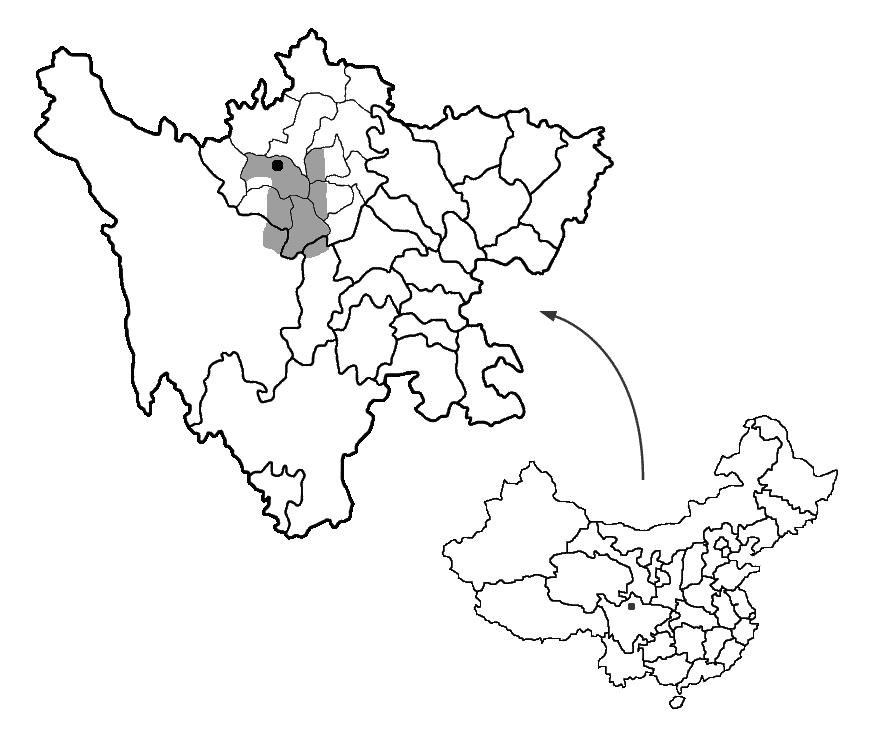
\includegraphics[width=0.5\textwidth]{carte.JPG}

\end{itemize}
\end{frame} 


 \begin{frame} 
 

   \begin{exe}
      \frametitle{Pronouns}
\ex \label{ex:nWGi.kAsWso}
\gll 
\ipa{nɤ-wa}  	\ipa{kɯ}  	``\rouge{\ipa{nɤʑo}} 	\bleu{\ipa{nɯɣi}}"  	\ipa{kɤ-sɯso}  	\ipa{kɯ}  	\ipa{kʰa}  	\ipa{ɯ-rkɯ}  	\ipa{ʁmaʁ}  	\ipa{χsɯ-tɤxɯr}  	\ipa{pa-sɯ-lɤt}  	\ipa{ɕti}  	\ipa{tɕe}  \\
\textsc{2sg.poss}-father \textsc{erg} \rouge{\textsc{2sg}} \bleu{come.back:\textsc{fact}}  \textsc{inf}-think \textsc{erg} house \textsc{3sg.poss}-side soldier three-circle \textsc{pfv:3$\rightarrow$3'-caus}-throw be.\textsc{affirmative}:\textsc{fact} \textsc{lnk}\\
\glt \textbf{Direct}: Your father, thinking ``\rouge{He} \bleu{is coming back}",   put three circles of soldiers around the house. 
\glt  \textbf{Indirect}: Your father, thinking that \rouge{you} are coming back,
 \end{exe}
  \end{frame} 
  
        \begin{frame} 
      \frametitle{Pronouns}
      The verb \ipa{sɯso} `think' is transitive, so the absence of ergative marking on \ipa{ɯʑo} `he' shows that this pronoun is the S of the complement clause, not the A of the main verb.
      
\begin{exe}
\ex
\gll  ``\rouge{\ipa{ɯʑo}}  	\ipa{χsɯ-sŋi}  	\ipa{χsɤ-rʑaʁ}  	\ipa{ma}  	\bleu{\ipa{mɯ-pɯ-rɤʑi-a}}"  	\ipa{ɲɯ-nɯ-sɯsɤm}  	\ipa{pjɤ-ŋu}  \\
\rouge{\textsc{3sg}} three-day  three-night apart.from \bleu{\textsc{neg-pst.ipfv}-stay-\textsc{1sg}} \textsc{ipfv-auto}-think[III] \textsc{evd.ipfv}-be \\
\glt    \textbf{Direct}: He was thinking ``\rouge{I} \bleu{have} only \bleu{stayed} for three days and three nights."
\glt    \textbf{Indirect}: He was thinking that \rouge{he} had only stayed for three days and three nights.
  \end{exe}
 \end{frame} 
 
 
%  \begin{frame} 
%\begin{exe}
%\ex
%\gll \ipa{tɕe}  	``\rouge{\ipa{tɕhi}}  	\bleu{\ipa{pɯ-sat-a}}"  	\ipa{nɯ}  	\ipa{mɯ-ko-rɤt}  	\ipa{kɯ,}  	``\ipa{tɯtɯrca}  	\ipa{kɯɕnɯz}  	\ipa{pɯ-sat-a.}"  	\ipa{ko-rɤt.}  \\
%\textsc{lnk} \rouge{what} \bleu{\textsc{pfv}-kill-\textsc{1sg}}  \textsc{dem} \textsc{neg-evd}-write \textsc{erg} together seven \textsc{pfv}-kill-\textsc{1sg} \textsc{neg-evd}-write \\
%\glt Direct: He did not write \rouge{what} he had killed,  he (just) wrote ``I killed seven (of them)."
%  \end{exe}
% \end{frame} 
 
   \begin{frame} 
   \frametitle{Possessive prefixes}
\begin{exe}
\ex
\gll  \ipa{tɕe}  	\ipa{ta-ʁi}  	\ipa{nɯ}  	\ipa{kɯ}  	``\rouge{\ipa{ɯ-pi}}  	\ipa{ɣɯ}  	\ipa{ɯ-sci}  	\bleu{\ipa{tu-nɤme-a}}  	\ipa{ra}" 	\ipa{ɲɤ-sɯso}  	\ipa{tɕe,}  	\\
\textsc{lnk}  \textsc{indef.poss}-younger.sibling \textsc{dem} \textsc{erg}  \rouge{\textsc{3sg.poss}-elder.sibling}  \textsc{gen} \textsc{3sg.poss}-revenge \bleu{\textsc{ipfv}-make[III]-\textsc{1sg}} have.to:\textsc{fact} \textsc{evd}-think \textsc{lnk} \\
\glt  \textbf{Direct}: The (younger) sister thought ``\bleu{I have to get revenge} on \rouge{my brother}".
\glt  \textbf{Indirect}:  The (younger) sister thought  to get revenge on \rouge{her brother}".
  \end{exe}
 \end{frame} 
 

    \begin{frame} 
       \frametitle{Possessive prefixes}
\begin{exe}
\ex
\gll   \ipa{tɤɕime}  	\ipa{nɯ}  	\ipa{kɯ}  	\ipa{pjɯ-tɯ-mtshɤm}  	\ipa{tɕe,}  	\ipa{nɯnɯ}  \rouge{\ipa{ɯ-kɯmtɕhɯ}}  	\ipa{nɯ}  	\bleu{\ipa{ju-ɣɯt-a}}  	\ipa{ŋu}  		\ipa{ɯ-kɯ-ti}  	\ipa{pjɤ-tu}  	\ipa{ndɤre,}  \\
girl \textsc{dem} \textsc{erg} \textsc{ipfv-conv:imm}-hear \textsc{lnk} \textsc{dem} \rouge{\textsc{3sg.poss}-toy} \textsc{dem} \bleu{\textsc{ipfv}-bring-\textsc{1sg}}  be:\textsc{fact} \textsc{3sg-nmlz}:S/A-say \textsc{evd.ipfv}-exist \textsc{lnk} \\
\glt   \textbf{Direct}: As soon as the girl heard it, that there was someone saying ``\bleu{I will bring} \rouge{your toy}".
\glt   \textbf{Indirect}: there was someone saying that he would bring \rouge{her toy}".
  \end{exe}
 \end{frame} 

 
     \begin{frame} 
        \frametitle{Possessive prefixes}
\begin{exe}
\ex
\gll   \rouge{\ipa{a-tʂɯnlɤn}}  	\bleu{\ipa{ɲɯ-nɯ-fsɯɣ-a}}  	\ipa{ɯ-ɲɯ-tɯ-sɯsɤm}  	\ipa{nɤ,}  	\ipa{nɯ}  	\ipa{tɤ-ste}  	\ipa{ti}  \ipa{ɲɯ-ŋu} \\
 \rouge{\textsc{1sg.poss}-favour} \bleu{\textsc{ipfv-auto}-pay.back-\textsc{1sg}} \textsc{cond-ipfv}-2-think[III] \textsc{lnk} \textsc{dem} \textsc{imp}-do.this.way[III] say:\textsc{fact} \textsc{testim}-be \\
 \glt    \textbf{Direct}: If you think ``\bleu{I will requite} the \rouge{favour} (which I received from \rouge{you})", do like that.
\glt    \textbf{Indirect}: If you want to requite the \rouge{favour} (which you received from \rouge{me}), do like that.
  \end{exe}
 \end{frame} 
 
 
 
 
 
  \begin{frame} 

\bibliographystyle{linquiry2} 
\bibliography{bibliogj}
 
 \end{frame} 
\end{document}
